\documentclass[conference, 11pt]{IEEEtran}

\usepackage[labelfont=bf]{caption} 
\captionsetup{labelfont=bf}
\usepackage{tcolorbox}
\usepackage{minted}
\usepackage{xcolor} % to access the named colour LightGray
\definecolor{LightGray}{gray}{0.9}
\usepackage{hyperref}
\usepackage{listings}
\usepackage{filecontents}
\usepackage{balance}
\usepackage{subfig}

\definecolor{bg}{gray}{0.95}

\lstset{
  basicstyle=\ttfamily,
  mathescape=true,
  frame=single,
  breaklines=true,
  numbers=left,
  numberstyle=\small,
  xleftmargin=2em,
  framexleftmargin=1.8em
}

\begin{document}

\makeatletter
\newcommand{\linebreakand}{
  \end{@IEEEauthorhalign}
  \hfill\mbox{}\par
  \mbox{}\hfill\begin{@IEEEauthorhalign}
}
\makeatother
\makeatletter
\patchcmd{\@maketitle}
  {\addvspace{0.5\baselineskip}\egroup}
  {\addvspace{-1\baselineskip}\egroup}
  {}
  {}
\makeatother

\title{VISION-DR: Visual Insights and Saliency Integrated Overlay Neural Network for \\Diabetic Retinopathy}

\author{
    \IEEEauthorblockN{Beyza Cavdar}
    \IEEEauthorblockA{
    Northeastern University\\
    Boston, Massachusetts, USA\\
    cavdar.b@northeastern.edu}
    \and
    \IEEEauthorblockN{Nihira Golasangi}
    \IEEEauthorblockA{
    Northeastern University\\
    Boston, Massachusetts, USA\\
    golasangi.n@northeastern.edu}
    \linebreakand
    \IEEEauthorblockN{Scott Perryman}
    \IEEEauthorblockA{
    Northeastern University\\
    Boston, Massachusetts, USA\\
    perryman.s@northeastern.edu}
    \and 
    \IEEEauthorblockN{Harrison Sun}
    \IEEEauthorblockA{
    Northeastern University\\
    Boston, Massachusetts, USA\\
    sun.har@northeastern.edu}
}

\maketitle
% \thispagestyle{empty}
\thispagestyle{plain}
% \pagestyle{empty}
\pagestyle{plain}
\begin{abstract}

Lorem ipsum dolor sit amet, consectetur adipiscing
elit. Praesent non accumsan purus. Pellentesque vel dig-
nissim nisi. Orci varius natoque penatibus et magnis dis
parturient montes, nascetur ridiculus mus.

\end{abstract}
\begin{IEEEkeywords}
Lorem, Ipsum, Dolor
\end{IEEEkeywords}

\section{Introduction}
Diabetic retinopathy is an eye disease associated with both Type 1 and Type 2 diabetes that causes damage to the blood vessels in the retina \cite{noauthor_diabetic_nodate}. Left untreated, diabetic retinopathy can cause permanent vision loss \cite{lee_epidemiology_2015}. The Center For Disease Control (CDC) estimates that there are 9.6 million people in the United States living with Diabetic Retinopathy, of whom 1.84 million have vision-threatening diabetic retinopathy \cite{noauthor_diabetic_2023}. Since diabetic retinopathy is caused by swelling and leaking in the vasculature, which is associated with elevated blood glucose over long periods of time, it is imperative that the disease be caught earlier rather than later \cite{hammes_diabetic_2011}. Notably, early-detection enables non-invasive treatments involving controlling blood glucose levels, blood pressure, and cholesterol levels \cite{stitt_progress_2016}. However, late-stage diabetic retinopathy treatments are generally more invasive, including photocoagulation, steroid injections, and vitrectomy \cite{stitt_progress_2016}. 

Diabetic retinopathy is typically divided into 5 stages: \textbf{0: No DR} - no hemorrhaging, microaneurysms, or abnormal vascularization occurs, \textbf{1: Mild Non-proliferative DR} - swelling in small blood vessels occurs, \textbf{2: Moderate Non-proliferative DR} - blood vessels become blocked, \textbf{3: Severe Non-proliferative DR} - ischemia occurs, blot hemorrhaging occurs, and abnormal vascularization may occur, and \textbf{4: Proliferative DR} - new, abnormal and fragile, blood vessels begin to grow in the eye \cite{yun_identification_2008}.

Our goal is to introduce a computer vision model that aids physicians in accurately diagnosing the various stages of diabetic retinopathy. This model aims to serve as a critical tool, enhancing the precision of clinical assessments and facilitating a more streamlined diagnostic process. By integrating visual data analysis, the model provides valuable support in clinical decision-making, offering physicians insights that are essential for monitoring disease progression over time. Ultimately, our goal is to equip healthcare providers with technology that not only improves diagnostic accuracy but also contributes to the longitudinal study of diabetic retinopathy, paving the way for better patient outcomes.

\section{Background}
Diabetic retinopathy is a progressive disease that necessitates early and accurate detection to prevent severe vision loss. With the increasing prevalence of diabetes worldwide, efficient and scalable diagnostic technologies are crucial. Computer vision has emerged as a powerful tool in this context, enabling the automated detection and classification of diabetic retinopathy.

Computer vision has become increasingly prevalent in medical diagnostics \cite{esteva_deep_2021}. Specifically for diabetic retinopathy, it typically involves the use of classifiers that categorize a single fundus image into one of five stages of the disease \cite{mateen_fundus_2019}. The VGG model, known for its robust feature extraction capabilities, is particularly favored in image recognition tasks \cite{mateen_fundus_2019, kaur_automated_2019, ha_image_2018, varshni_pneumonia_2019, chaib_deep_2017, lu_feature_2017, majib_vgg-scnet_2021, tammina_transfer_2019}. It effectively identifies key indicators of diabetic retinopathy such as microaneurysms, exudates, hemorrhages, and abnormal vascularization \cite{hwang_optical_2015-2}. Existing applications of this model have achieved accuracies exceeding 85\% in diagnosing the condition \cite{noauthor_diabetic_nodate}.

Despite these advancements, the opaque ``black box'' nature of deep learning models poses a significant barrier to their adoption in clinical settings \cite{guidotti_survey_2018}. Traditionally, the decision-making processes of these models are not transparent, leaving physicians without a clear understanding of why certain decisions were made \cite{guidotti_survey_2018}. To overcome this challenge, researchers have developed explainability techniques like Grad-CAM \cite{selvaraju_grad-cam_2017}. These techniques provide visual explanations by highlighting influential regions in the images at one of the final layers of the network. This not only helps bridge the gap between model decision-making and user interpretability but also supports physicians in integrating their clinical expertise with model suggestions for better-informed decision-making.

\section{Problem Formulation}
The goal of our project is to advance the diagnosis of diabetic retinopathy, a leading cause of blindness among adults worldwide, by implementing a dual-purpose computer vision algorithm. This algorithm is designed not only to improve diagnostic accuracy but also to enhance transparency in the diagnostic process. Current methods for detecting and assessing diabetic retinopathy depend heavily on the manual examination of retinal images by skilled clinicians. These methods are often limited by the availability of experts and can suffer from subjective variability in diagnosis. As the prevalence of diabetes increases globally, there is an urgent need for a more scalable and consistent approach to diagnosing this vision-threatening condition.

Our objectives are twofold. Firstly, we aim to accurately classify the severity of diabetic retinopathy across its spectrum, from mild to severe stages. The ability to classify with high precision is crucial as it directly informs treatment options and management strategies, potentially leading to better patient outcomes. Secondly, we seek to increase the accountability and trustworthiness of AI in medical diagnostics by generating saliency maps. These maps are intended to visually represent the critical features within the retinal images that influence the AI's decision-making process. By doing so, we aim to provide clinicians and patients with clear, visual explanations of the AI's diagnoses, promoting transparency and understanding.

In summary, our work seeks to address the significant challenge of scaling diabetic retinopathy diagnostics while maintaining the quality and reliability expected in healthcare. By achieving these goals, we anticipate that the confidence in AI-assisted diagnostics will be significantly bolstered, leading to wider acceptance and use of these technologies in clinical settings. This approach not only promises to enhance the capacity for early detection and treatment of diabetic retinopathy but also sets a precedent for the application of AI in other areas of medical imaging and diagnosis.

\section{Methodology}
\begin{figure*}[h]
  \centering
  \begin{minipage}{\textwidth}
    \centering
    \begin{lstlisting}[]
    BEGIN
      // Load Pretrained Weights
      vgg_model $\leftarrow$ load_model("VGG16", pretrained=True)

      // Unfreeze all layers for training
      FOR layer IN vgg_model.parameters()
        layer.requires_grad $\leftarrow$ True
      END FOR

      // Modify classifier structure
      vgg_model.classifier[6] $\leftarrow$ Sequential(
        Linear(4096, 1024),
        ReLU(),
        Dropout(0.5),
        Linear(1024, 1),
        Sigmoid()
      )

      // Set device
      device $\leftarrow$ if GPU_available() then "cuda:0" else "cpu"
      vgg_model.to(device)

      // Loss function
      criterion $\leftarrow$ Cross_Entropy_Loss()

      // Use Adam Optimizer
      optimizer $\leftarrow$ Adam(vgg_model.classifier.parameters(), lr=0.001)
    END
    \end{lstlisting}
    \caption{Pseudocode for adapting a pre-trained VGG-16 model for Diabetic Retinopathy classification.}
    \label{fig:vgg16}
  \end{minipage}%
\end{figure*}

The dataset we use is the Kaggle Diabetic Retinopathy Detection Dataset \cite{emma_dugas_diabetic_2015}. The dataset consists of over 35,000 high resolution retina images captured with a fundus camera \cite{emma_dugas_diabetic_2015, mateen_fundus_2019}. All of the images are labeled by clinicians into 5 numbered classes corresponding to severity. The data is structured into training and testing files as well as a file delineating training and testing labels.

We have constructed a classifier employing the VGG-16 architecture, which is a convolutional neural network with 16 layers \cite{simonyan_very_2015}. As outlined in \autoref{fig:vgg16}, our approach starts with loading the VGG-16 model pre-equipped with trained weights. Subsequently, we enable training on all layers by unfreezing their weights. The VGG architecture utilizes 3x3 convolutional filters and max-pooling to minimize the model's complexity and the number of parameters needed. The classifier's configuration is altered to include a linear layer, a ReLU activation function, a dropout rate of 0.5 to prevent overfitting, another linear layer, and a sigmoid activation to produce a probability output. The model is trained using cross-entropy loss and optimized with the Adam optimizer with a learning rate of 0.001  \cite{zhang_generalized_2018, kingma_adam_2017}.

Following the training and optimization of the VGG-16 model for diabetic retinopathy detection, we employ Gradient-weighted Class Activation Mapping (Grad-CAM) to enhance the interpretability of the model’s predictions \cite{selvaraju_grad-cam_2017}. Grad-CAM is a visualization technique that highlights the regions in the input image that are important for predictions from convolutional neural networks. This method uses the gradients of the output of the final convolutional layer to produce a coarse localization map highlighting the important regions in the image for predicting the concept.

To implement Grad-CAM, we first import the best-performing VGG-16 model trained on the diabetic retinopathy dataset. We then focus on the activations and gradients of the final convolutional layer, as this layer captures the most complex features in the image that are crucial for making the final decision. By computing the gradient of the output category with respect to the feature maps of the final convolutional layer, and then pooling these gradients over the spatial dimensions, we create a weighted map of the important features. This weighted feature map is then used to create a heatmap by performing a weighted combination of the feature maps, followed by a rectified linear transformation. Finally, this heatmap is superimposed on the original image to visually represent the areas most significant for the model’s classification decision, providing insights into what the model is considering important in diagnosing diabetic retinopathy. This method not only aids in verifying the model's focus areas but also enhances trust and understanding in its diagnostic decisions, making it a powerful tool for medical imaging analysis.



\section{Results \& Discussion}
\begin{figure*}[h]
  \centering
  \begin{minipage}{.5\textwidth}
    \centering
    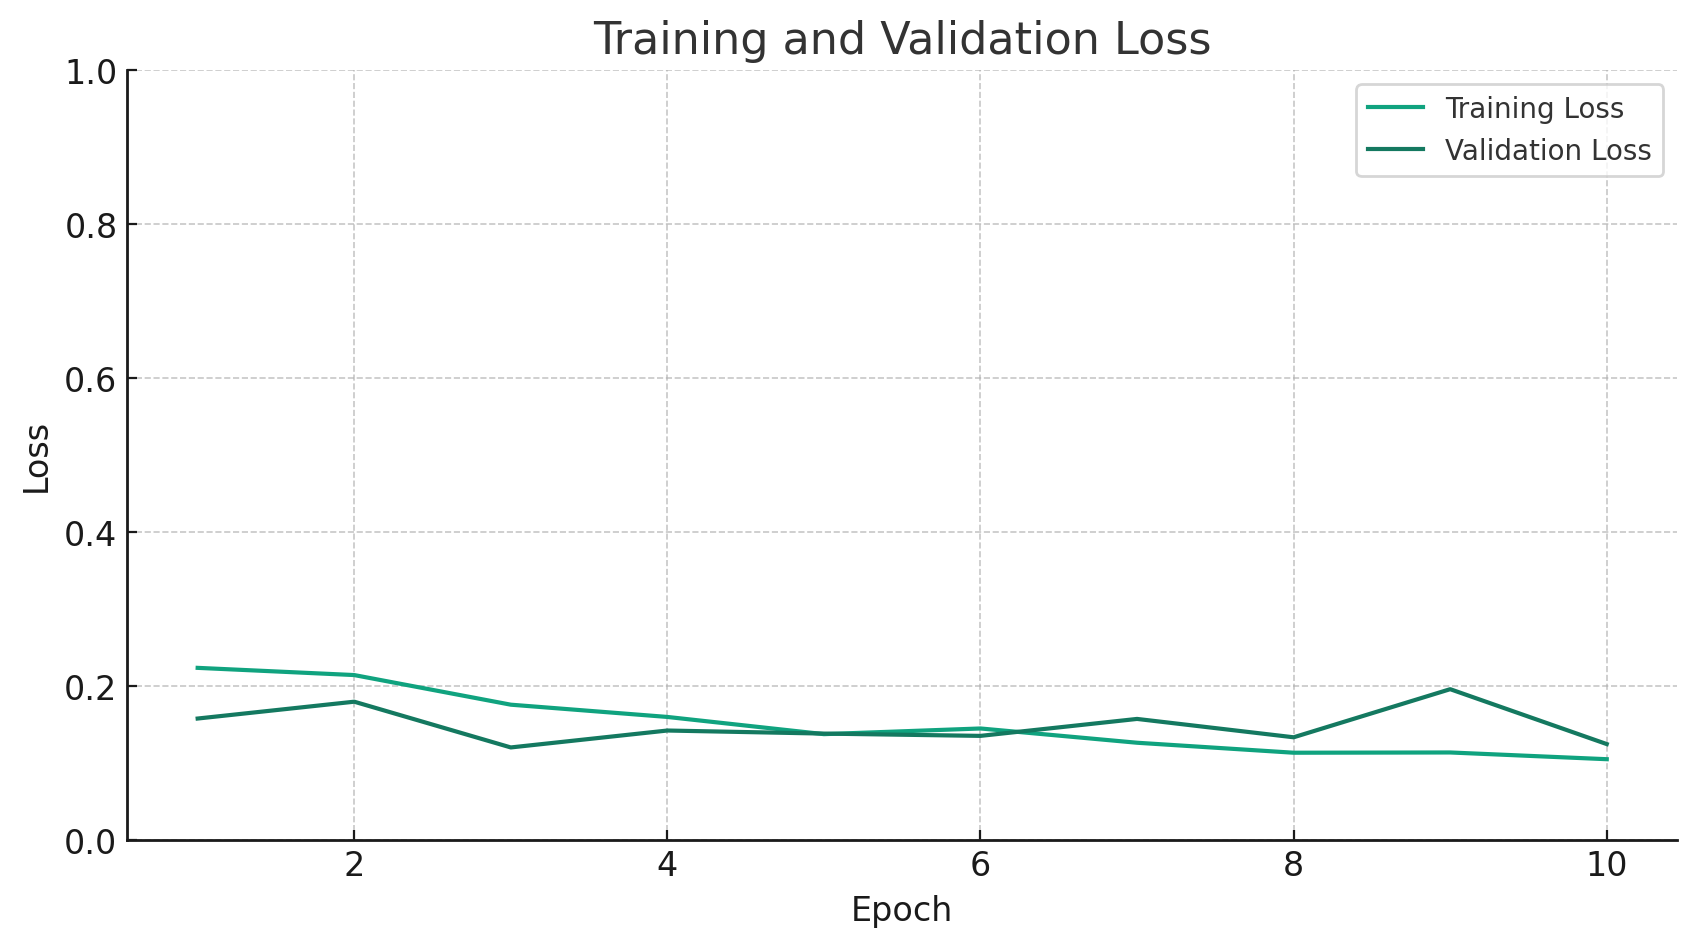
\includegraphics[scale=0.4]{Images/Loss.jpg}
    \caption{Loss per Epoch}
    \label{fig:loss}
  \end{minipage}%
  \begin{minipage}{.5\textwidth}
    \centering
    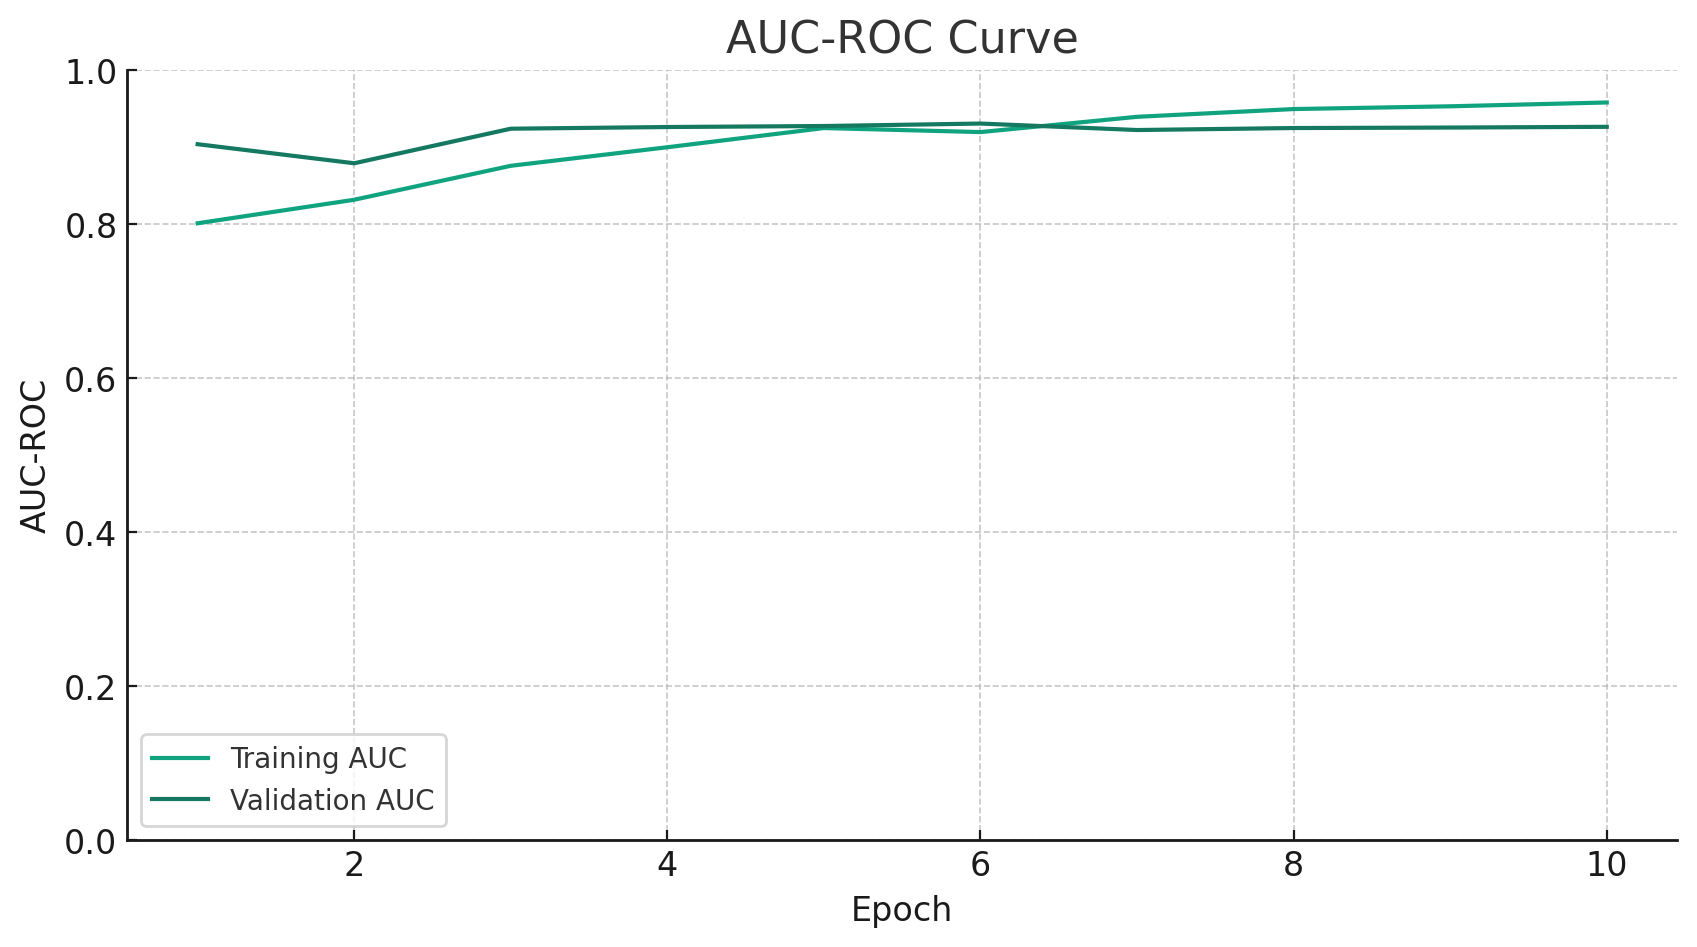
\includegraphics[scale=0.4]{Images/AUC-ROC.jpg}
    \caption{AUC-ROC Score per Epoch}
    \label{fig:auc-roc}
  \end{minipage}
\end{figure*}

The goal of this project was to accurately classify the severity of diabetic retinopathy in fundus camera images and to generate a saliency map highlighting the image regions influencing the classification decision. We evaluated model performance using cross-entropy loss and the Area Under the Receiver Operating Characteristic Curve (AUC-ROC). Due to significant class imbalance, we chose AUC-ROC over accuracy as a performance metric. Since AUC-ROC remains unaffected by skewed class distributions, it provides a more reliable indicator of model efficacy than accuracy. Additionally, the AUC-ROC curve is influenced by the balance between sensitivity and specificity, ensuring that the abundance of Class 0 cases does not skew the performance metric.

\autoref{fig:loss} illustrates the training and validation loss trends. Notably, at around 10 epochs, both training and validation losses converge to approximately 0.15. While the training loss continues to decrease, the validation loss begins to fluctuate after a few epochs. To prevent overfitting and manage computational resources efficiently, we limited our training to 10 epochs.

\autoref{fig:auc-roc} displays the AUC-ROC for both training and validation sets, which begin to plateau at about the fifth epoch, peaking near 0.9. This indicates a 90\% probability that the model accurately distinguishes between the two classes, confirming the model's robust performance in assessing the severity of diabetic retinopathy and achieving our primary objective.

Our secondary objective involves visually identifying the critical areas influencing the model's decisions. \autoref{fig:dr0} presents a saliency map for an image classified as Class 0 (No Diabetic Retinopathy), where the focus is primarily on three regions. The top left and bottom left corners are examined for notches indicating mirrored images. The right-hand focus assesses the blood vessels for abnormal vascularization and hemorrhaging. Conversely, \autoref{fig:dr4} shows a saliency map for Class 4 (Proliferative Diabetic Retinopathy), with particular attention to neovascularization driven by angiogenesis and hemorrhaging. Notably, the model disregards a large dark spot in the upper left quadrant, which we identified as a choroidal nevus — a benign, commonly occurring pigmented lesion unrelated to diabetic retinopathy \cite{noauthor_distinguishing_2012}. This discernment demonstrates the model's capability to distinguish between relevant and unrelated features, which we consider satisfactory for our second objective. However, a comprehensive assessment of the model's performance across various features would require extensive clinical annotation.

\begin{figure*}[t]
  \centering
  \begin{minipage}{\textwidth}
    \centering
    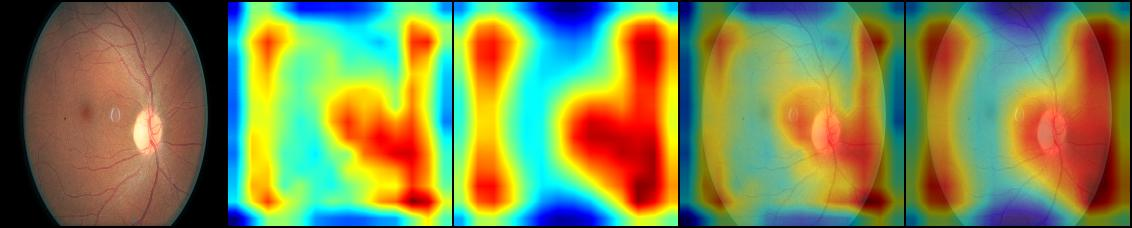
\includegraphics[scale=0.4]{Images/20_left.jpeg}
    \caption{Saliency Map for an Image with No Diabetic Retinopathy}
    \label{fig:dr0}
  \end{minipage}%
\end{figure*}

\begin{figure*}[t]
  \centering
  \begin{minipage}{\textwidth}
    \centering
    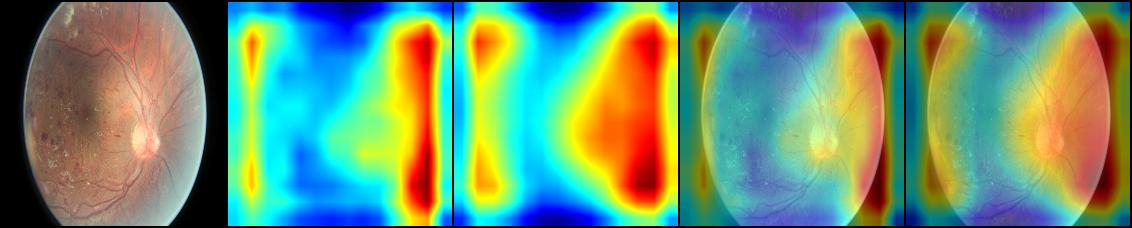
\includegraphics[scale=0.4]{Images/16_left.jpeg}
    \caption{Saliency Map for an Image with Proliferative Diabetic Retinopathy}
    \label{fig:dr4}
  \end{minipage}%
\end{figure*}

\section{Future Work}
A key area of interest is the development of an image segmentation system that can delineate detailed structures within fundus images. Current limitations stem from the precision required in labeling segmentation masks, a task that demands specialized medical expertise. Collaborating with clinicians to label these fine masks accurately would enable us to enhance our model's understanding of the spatial relationships and exact boundaries of lesions associated with diabetic retinopathy.

Moreover, integrating segmentation with our existing classification model could significantly refine its performance. Segmentation masks could serve not only to validate the areas of interest identified by the saliency maps but also to quantify aspects such as the area affected by different classes of retinopathy. This quantitative data could be invaluable in training more sophisticated machine learning models that consider the extent and specific locations of retinopathy signs as factors in their predictions.

Another promising direction involves tracking the progression of diabetic retinopathy over time. By developing algorithms that analyze sequential fundus images of the same patients, we can gain insights into the evolution of the disease. This longitudinal analysis would allow for more personalized and timely treatment decisions, potentially slowing or even reversing the progression of retinopathy.

Finally, integrating findings from existing literature into our models through the use of regularization techniques based on prior knowledge stands to significantly improve model performance and reliability. By incorporating constraints derived from the extensive literature on diabetic retinopathy and related pathologies, we can guide the learning process of our models to adhere more closely to clinically observed patterns. This regularization could help mitigate the effects of overfitting and improve generalization to new, unseen data by aligning our model's inferences with established medical knowledge.

\section{Conclusion}
This project has demonstrated the potential of computer vision models in enhancing the diagnosis of diabetic retinopathy through fundus camera images. By employing the AUC-ROC metric, which is particularly effective in conditions of class imbalance, the model achieved a robust ability to distinguish between different severity levels of retinopathy. Furthermore, the generation of saliency maps provided visual confirmation of the regions in the images that influenced the model's decisions, highlighting the model's capacity to identify clinically relevant features.

The model shows strong predictive performance and the insights gained from the saliency maps pave the way for more intricate explorations into image-based diagnostic processes. Future efforts could focus on advancing towards image segmentation to gain more detailed diagnostic information and on leveraging sequential image data to track the progression of retinopathy over time. Additionally, incorporating medical expertise into the labeling process and integrating established clinical knowledge into machine learning models through regularization would enhance the accuracy and reliability of diagnostic tools.

As we continue to bridge the gap between technical capabilities and clinical needs, the prospect of AI-driven tools becoming a staple in diagnostics is increasingly feasible. These tools promise not only to enhance diagnostic precision but also to enable earlier interventions, potentially altering the course of diabetic retinopathy for countless patients. 

\bibliographystyle{IEEEtran}
\bibliography{references}

\newpage
\onecolumn
\appendix
Lorem ipsum dolor sit amet, consectetur adipiscing elit. Praesent non accumsan purus. Pellentesque vel dignissim nisi. Orci varius natoque penatibus et magnis dis parturient montes, nascetur ridiculus mus. Cras maximus ex id efficitur molestie. Mauris nec magna eget purus placerat fringilla sagittis vitae enim. Praesent mauris metus, ullamcorper et fermentum vitae, pretium et magna. Nam vehicula tempus eros. In vel fringilla mi. Etiam accumsan elit eu est lobortis, a volutpat lectus varius.

In quis ipsum a neque efficitur dictum in in sem. Suspendisse potenti. Nullam a ante vitae orci ultrices condimentum sed ut velit. Sed dictum, lorem quis feugiat semper, ex metus sagittis libero, nec sagittis lorem metus pellentesque ex. Vestibulum justo felis, sollicitudin id aliquet sed, accumsan vitae ipsum. Aliquam varius libero nec turpis imperdiet, in sagittis dui convallis. Nullam sit amet est mi.

Quisque diam sem, pretium a consectetur ac, varius eu enim. Pellentesque quam enim, pellentesque eget faucibus non, faucibus eget justo. Nam commodo faucibus gravida. Orci varius natoque penatibus et magnis dis parturient montes, nascetur ridiculus mus. Suspendisse dignissim magna eget tellus efficitur, id ornare est bibendum. Curabitur posuere suscipit hendrerit. Ut vel dignissim erat. Ut id ex vulputate arcu gravida interdum. Vivamus ut turpis nec nunc tincidunt fringilla vitae id est. Proin fringilla risus nec dui ornare commodo. Vestibulum lobortis augue nisi, sit amet porttitor risus hendrerit ut. Morbi dictum imperdiet lacus, eget dapibus justo. Etiam risus nisl, maximus ut dui ac, aliquam auctor ante. Proin id mauris tristique, euismod lorem ut, pulvinar nibh. Praesent vel semper leo.
\end{document}
